\documentclass[../../main.tex]{subfiles}
\begin{document}
\setcounter{footnote}{0} 
\newcommand{\rom}[1]{\uppercase\expandafter{\romannumeral #1\relax}}


\chapter{Metallocage Catalysis}

\section{Overview}

Arguably, biological catalysts -- referred to as enzymes -- are the best catalysts known. They operate in safe and abundant solvent (water), are highly active at room temperature or close to it and are highly selective. While \emph{de-novo} enzyme design is a promising and active area of research, laborious directed-evolution -- random mutation of amino acids and selection -- is generally required.\cite{Vller2020} Metallocages (\figurename{ \ref{fig::cage_overview_1}}) offer a promising alternative, with defined cavities, broadly predictable self-assembly and, therefore, easily tunable micro-environments, they provide a simpler approach to achieve enzyme-like catalytic properties.\cite{Sepehrpour2019}

\begin{figure}[h!]
	\vspace{0.4cm}
	\centering
	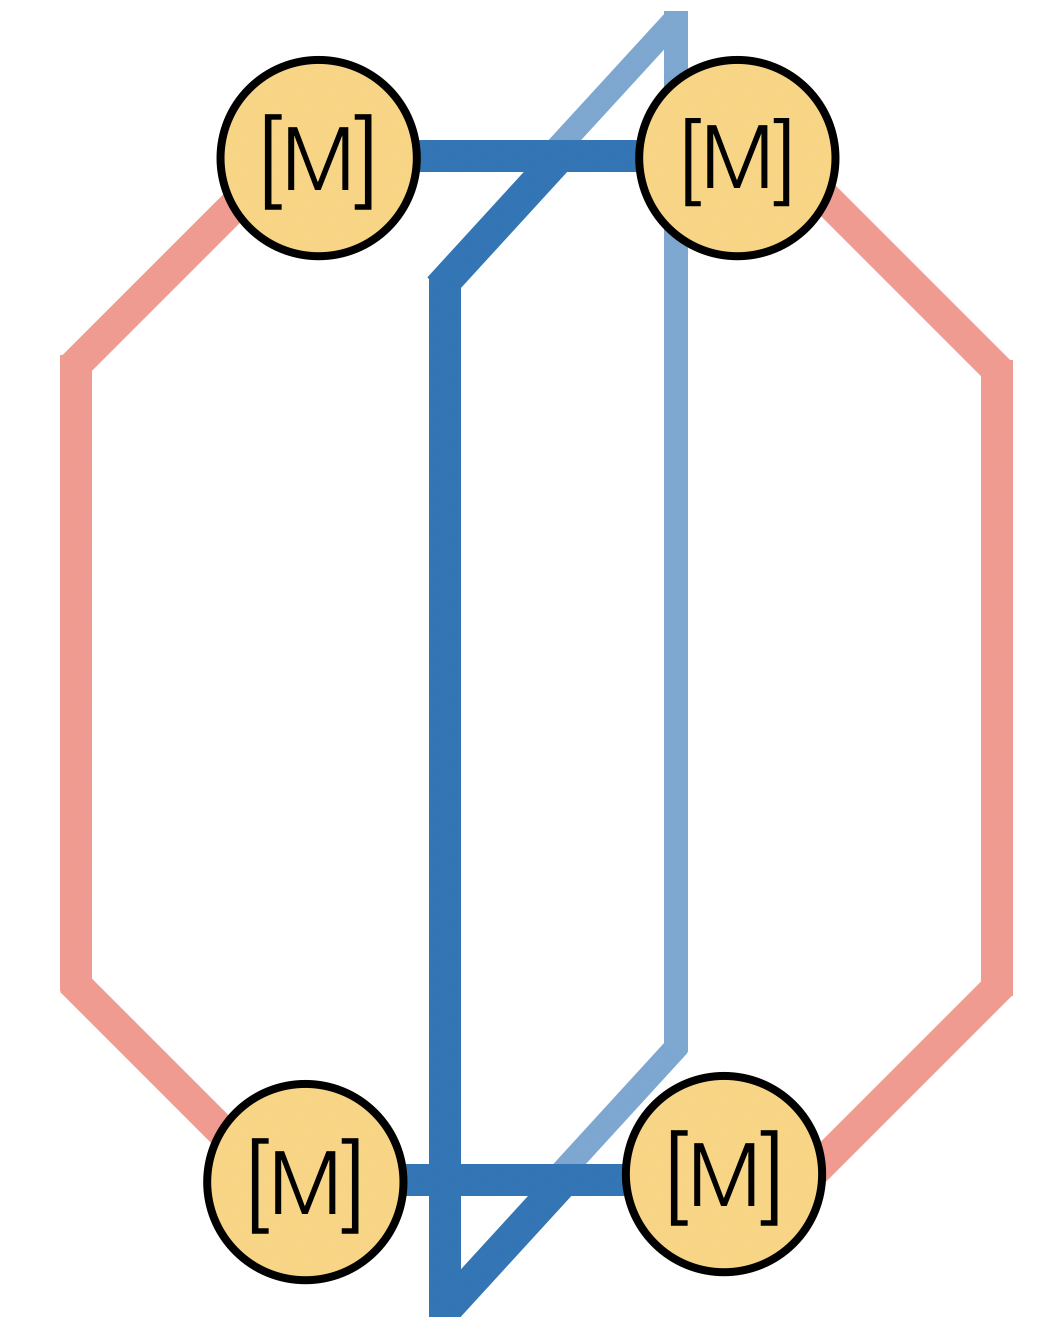
\includegraphics[width=4.5cm]{3/overview/figs/fig1/fig1}
	\vspace{0.3cm}
	\hrule
	\caption{Example metallocage structure with an M$_4$L$_1$L$'_1$ topology, where [M] is a metal fragment e.g. Au(I) or PdX$_2$.}
	\label{fig::cage_overview_1}
\end{figure}

Understanding how these metallocages can act as catalysts is thus an important step to rationally design catalytic metallocages with improved activity and selectivity. Manuscript \rom{1} focuses on understanding how an M$_2$L$_4$ construct catalyses a broad class of Diels-Alder reactions as shown experimentally by Lusby and co-workers in 2018.\cite{MartCentelles2018} The cages' flexibility, their cationic charge positioning, and ability to accommodate a guest are found to afford catalytic activity. En-route to these findings, the absolute and relative binding affinities and the catalytic ranking for a set of cages and substrates were all accurately reproduced by the computational approaches. These results suggest that more active catalysts could be developed by (1) increasing the effective charge of the metal sites; (2) reducing the steric clash between the substrate and cage upon translation to the exterior of the cavity and perhaps, (3) developing a cage large enough to accommodate both substrates (while still maintaining low product affinity, thus inhibition).

With an understanding of the catalytic mechanism for the metallocage a strategy to propose new catalysts is required. One such approach is to use chemical intuition and invest resources in setting up and analysing the calculations to minimise both the transition state barrier from the bound substrate and the binding energy of the product. An alternative approach would be to employ high-throughput virtual screening (HVTS). Towards this goal, Manuscript \rom{2} proposes a method and presents command-line (\emph{cgbind} Python module) and graphical ({\url{http://cgbind.chem.ox.ac.uk/}} web app)  implementations.

The graphical web-app was developed as a simple user-facing front-end to the Python module which currently provides only a subset of features but, nevertheless, is used for rapid visualisation of potential new metallocages for five architectures.\footnote{Private correspondence with the Lusby (University of Edinburgh), Craig (University of Strathclyde) and Zysman-Colman (University of St. Andrews) groups.} Behind the scenes \emph{cgbind} attempts to construct a metallocage by efficiently searching the space of donor atoms and conformations for possible metallocages. Distinct from other approaches\cite{Turcani2018} no hard-coded templates are defined but are rather automatically extracted from crystal structures. The Python module has been used within the Duarte group for a year or so for constructing, analysing and has started to be used to perform cage screening for catalytic proficiency.

\clearpage
\end{document}